\section{Horizon Length}

In order to determine what horizon length is needed to optimize the path, several paths were optimized with horizon lengths varying from $10$ to $140$, spaced by $10$. A piecewise linear and a curved $45\degree$ turn was optimized with the different horizon lengths. The resulting path flown by the UAV is shown in Figure \ref{fig:horizon_uav_position}, and the resulting camera position can be seen in Figure \ref{fig:horizon_camera_position}.

The results for the two paths are very similar, and longer horizon length seems to be synonymous with better tracking of the ground path. The MPC compensates for the sideways shift in the camera position cause by the roll angle by initiating the turn earlier, and the aircraft levels out from the turn later for the same reason.

For the shorter horizon lengths the MPC runs into problems because it hasn't planned far enough ahead when the turn begins. As the path starts turning the aircraft is still straight above it. At this point it is too late to start altering the aircrafts position to ensure that the camera footprint stays on the path, so the MPC creates a roll angle in the opposite direction of the path so that the camera continues to move in the direction of the path. This in turn leads to the aircraft turning left, worsening the situation and making the problem more and more difficult. In some cases this causes the roll angle to become very high, causing the MPC to lose control and the aircraft loses height.

%% Position figures

\begin{figure}
	\makebox[\textwidth][c]{
	\subfloat[Subfigure 1][Linear $45\degree$ turn.]{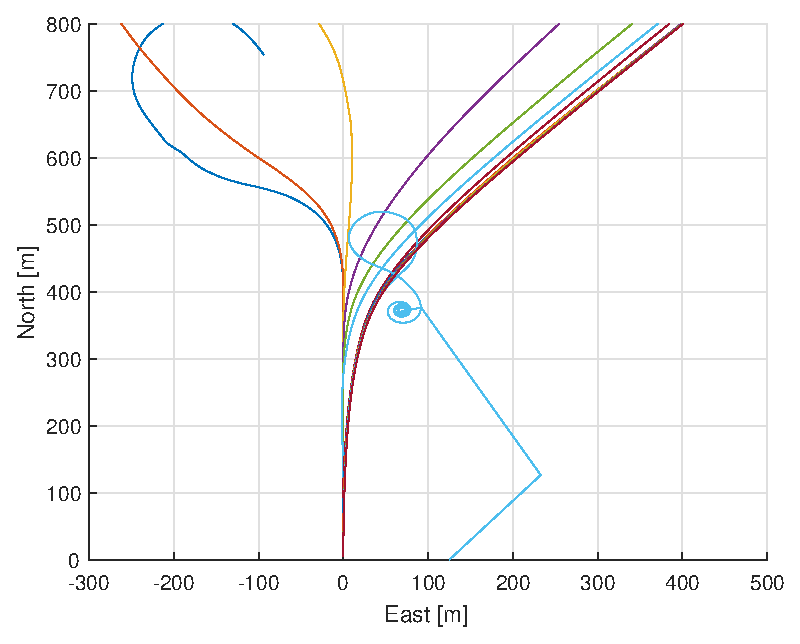
\includegraphics[width=0.8\textwidth, keepaspectratio=true]{../../results/opt/horizon/lin_45deg/fig/uav_position.eps}
	\label{fig:horizon_bad}}}
	\qquad
	\makebox[\textwidth][c]{
	\subfloat[Subfigure 2][Curved $45\degree$ turn with $200$m radius.]{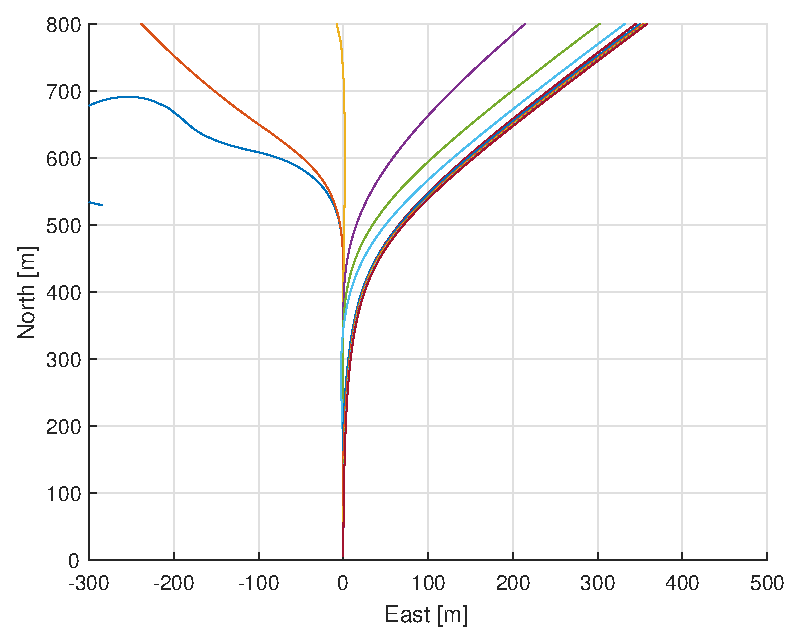
\includegraphics[width=0.8\textwidth, keepaspectratio=true]{../../results/opt/horizon/cur_45deg_200m/fig/uav_position.eps}}}
	\caption{The position of the UAV during the two turns with horizon lengths varying from 10 to 140.}
	\label{fig:horizon_uav_position}
\end{figure}


%% Camera position
\begin{figure}
	\makebox[\textwidth][c]{
	\subfloat[Subfigure 1][Linear $45\degree$ turn.]{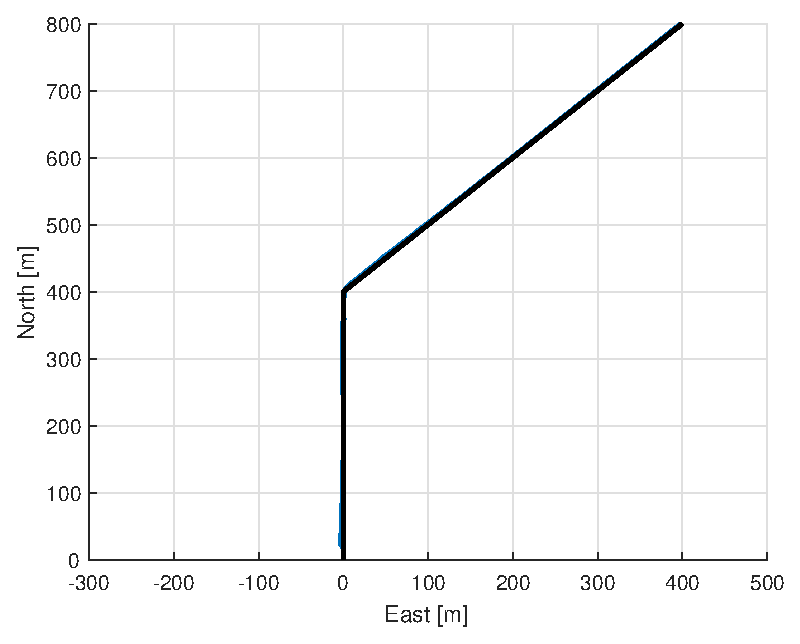
\includegraphics[width=0.8\textwidth, keepaspectratio=true]{../../results/opt/horizon/lin_45deg/fig/camera_position.eps}
	\label{fig:camera_horizon_bad}}}
	\qquad
	\makebox[\textwidth][c]{
	\subfloat[Subfigure 2][Curved $45\degree$ turn with $200$m radius.]{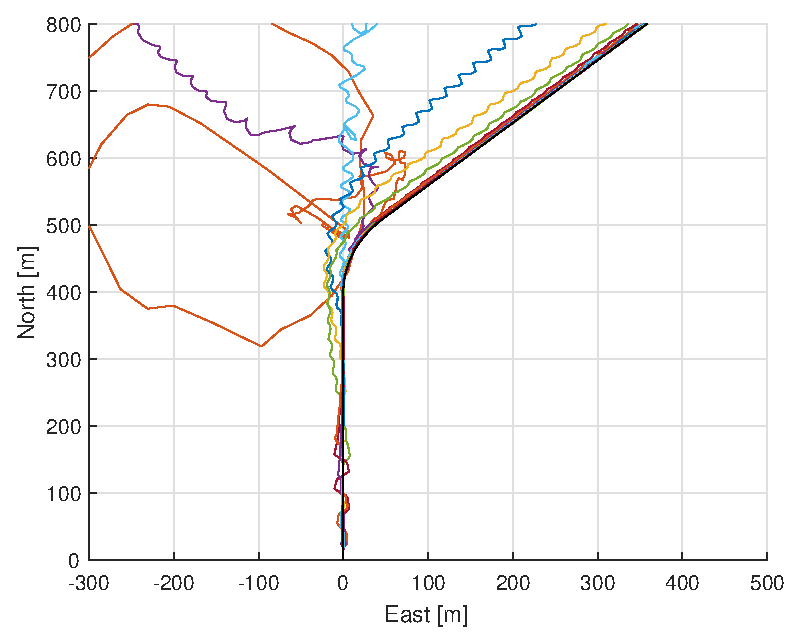
\includegraphics[width=0.8\textwidth, keepaspectratio=true]{../../results/opt/horizon/cur_45deg_200m/fig/camera_position.eps}}}
	\caption{The camera position during the two turns with horizon lengths varying from 10 to 140.}
	\label{fig:horizon_camera_position}
\end{figure}


%% Duration
\begin{figure}
	\makebox[\textwidth][c]{
	\subfloat[Duration]{\includegraphics[width=0.5\textwidth, keepaspectratio=true]{../../results/opt/horizon/duration_both.eps}
	\label{fig:horizon_duration}}
	\qquad
	\subfloat[Mean error]{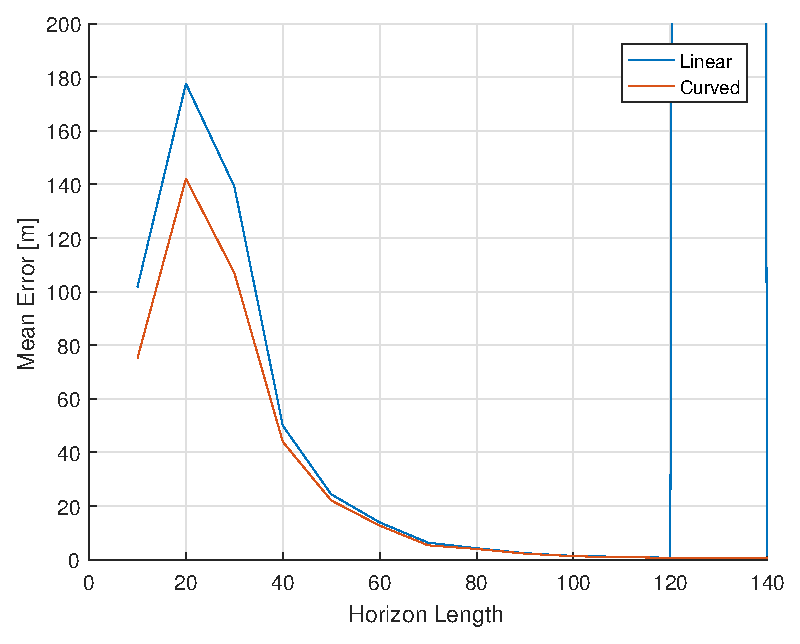
\includegraphics[width=0.5\textwidth, keepaspectratio=true]{../../results/opt/horizon/error_both.eps}
	\label{fig:horizon_mean}}}
	\caption{Duration of interval for varying horizon lengths, and the mean error.}
\end{figure}

Upon closer inspections it can be seen that when the horizon length reaches $90$, there are no more big unwanted motions in the system. As the horizon length reaches $110$ the optimized paths are almost identical, and as can be seen in Figure \ref{fig:horizon_mean}, there is very little precision to gain from increasing the horizon length. The optimization is time consuming, and as seen in Figure \ref{fig:horizon_duration} the time it takes to optimize the paths increases exponentially. For these reasons a horizon length of $110$ will be used for the rest of the simulations, as this gives an accurate path tracking for a relatively short computation time.

One result to take specific note of is the light blue UAV path in Figure \ref{fig:horizon_bad}. This path is generated when the horizon length is $130$, and is clearly not a solution to the optimization problem. There are no simple explanations for why this excact horizon length returns a bad result, as both lengths shorter and longer retunrn good results. One explanation may be that this excact horizon length with this excact discretized path gives to a very unfortunate set of waypoints. This result has been removed from the camera position shown in Figure \ref{fig:camera_horizon_bad}, as it made it difficult to see the other correct results.